\documentclass[11pt]{beamer}
\usepackage[utf8]{inputenc}
\usepackage[T1]{fontenc}

% Better hyphenation etc.
\usepackage{microtype}

% Define subfigures
\usepackage{subcaption}
\captionsetup{compatibility=false}

% Include images
\usepackage{graphicx}

% Place things at absolute positions
\usepackage[absolute,overlay]{textpos}

% Disable navigation buttons
\beamertemplatenavigationsymbolsempty

% Hide figure caption prefix
\setbeamertemplate{caption}{\raggedright\insertcaption\par}

% Insert title pages at the beginning of a section
\AtBeginSection[]{
  \begin{frame}
  \vfill
  \centering
  \Huge{\insertsectionhead}
  \vfill
  \end{frame}
}

\begin{document}

\begin{frame}
  \begin{center}
    
\includegraphics[width=80pt]{logo}\\

    \vspace{4em}

    {\LARGE Turbulent Flow Simulation on HPC-Systems}

    \vspace{2em}

    {\small Marten Lienen, Peter M\"unch, Walter Simson, Josef Winter}
  \end{center}
\end{frame}

\section{Instrumentation with ScoreP}

\section{Binary Data Output with HDF5}

\section{PETSc-Optimization}

\begin{frame}
  \frametitle{Automation}
  \begin{textblock}{8}(0.5,3)
    
\includegraphics[width=\textwidth]{petsc/python-logo}\\
  \end{textblock}

  % Option value combinations
  \begin{textblock}{6}(8.5,2)
    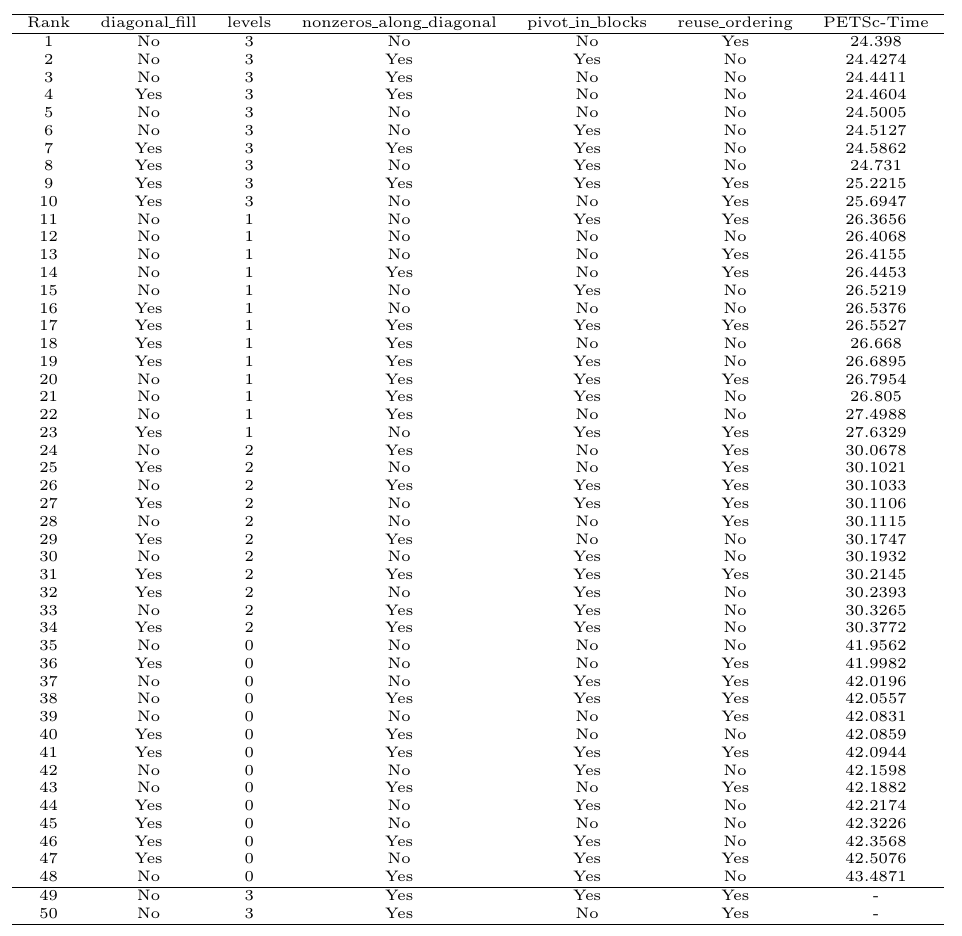
\includegraphics[width=\textwidth]{petsc/options-1x1}
  \end{textblock}
  \begin{textblock}{6}(9.5,7)
    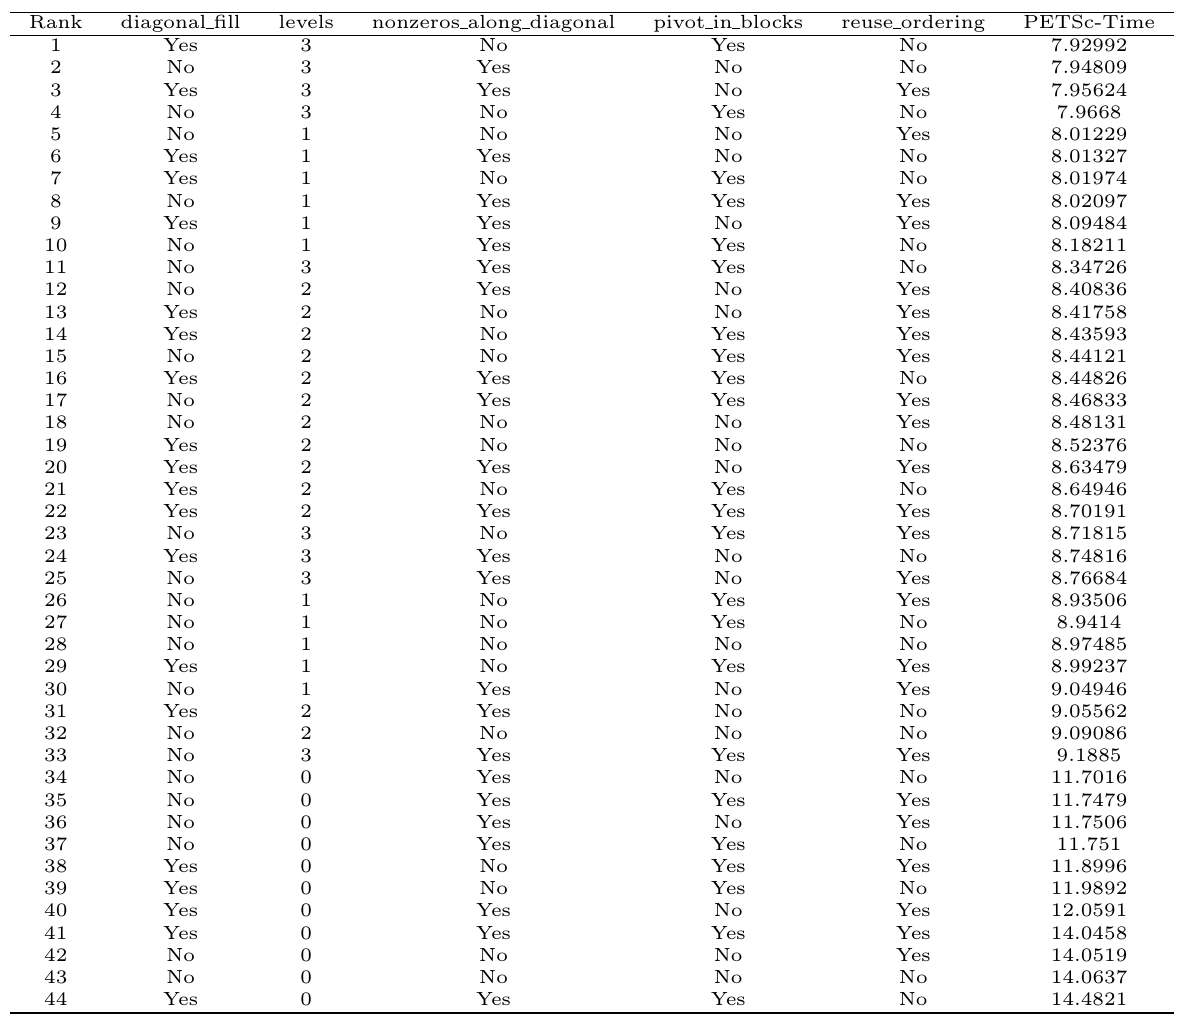
\includegraphics[width=\textwidth]{petsc/options-16x2}
  \end{textblock}

  % Solver/preconditioner combinations
  \begin{textblock}{6}(1,7)
    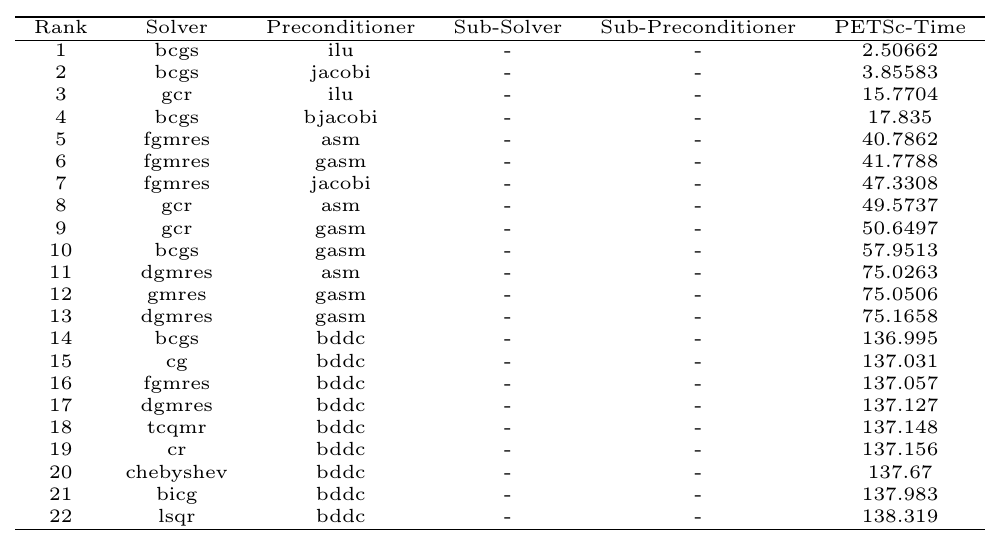
\includegraphics[width=\textwidth]{petsc/combinations-1x1}\\
  \end{textblock}
  \begin{textblock}{6}(3.5,8)
    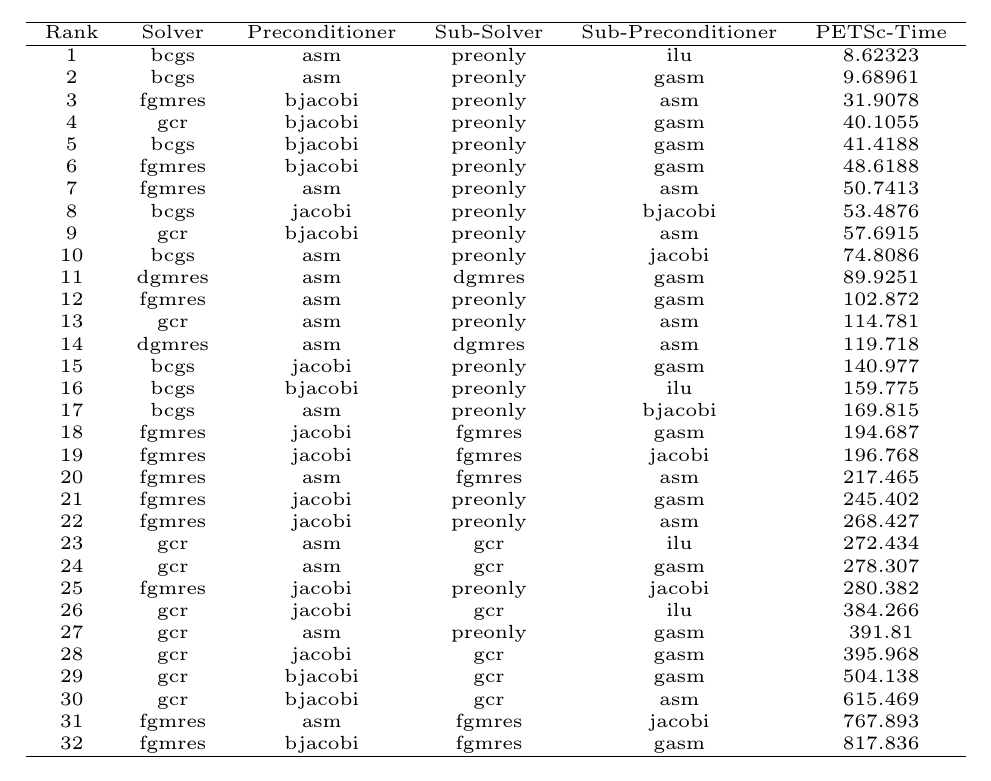
\includegraphics[width=\textwidth]{petsc/combinations-16x2}\\
  \end{textblock}
  \begin{textblock}{6}(2,10)
    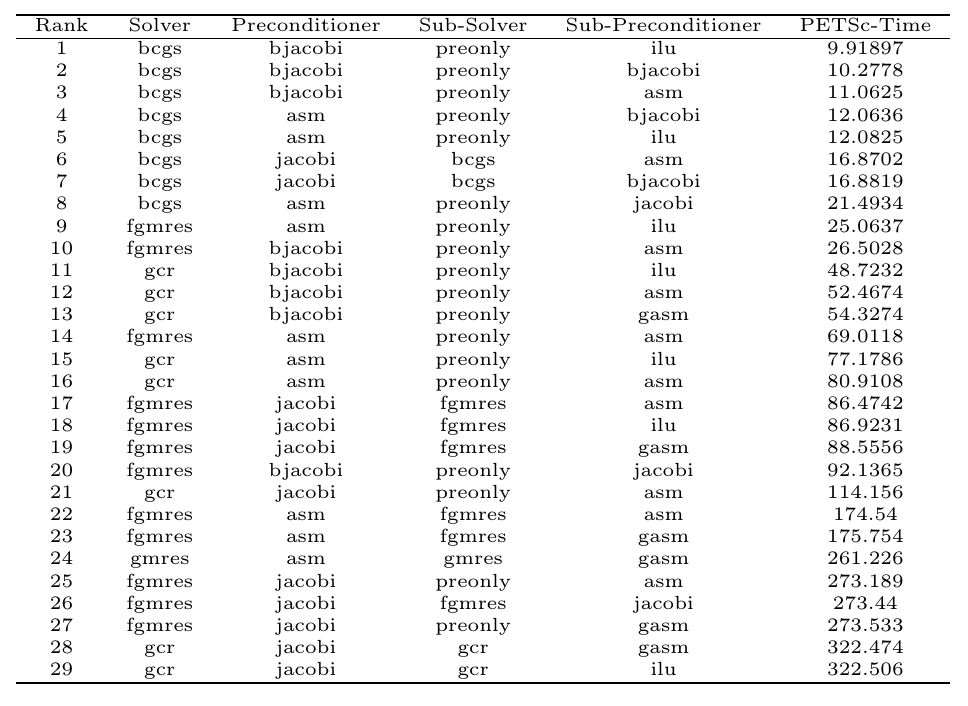
\includegraphics[width=\textwidth]{petsc/combinations-4x1}\\
  \end{textblock}
\end{frame}

\begin{frame}
  \frametitle{Scale Testing a DNS Case}
  \begin{figure}[h]
    \centering
    \begin{subfigure}{0.45\textwidth}
      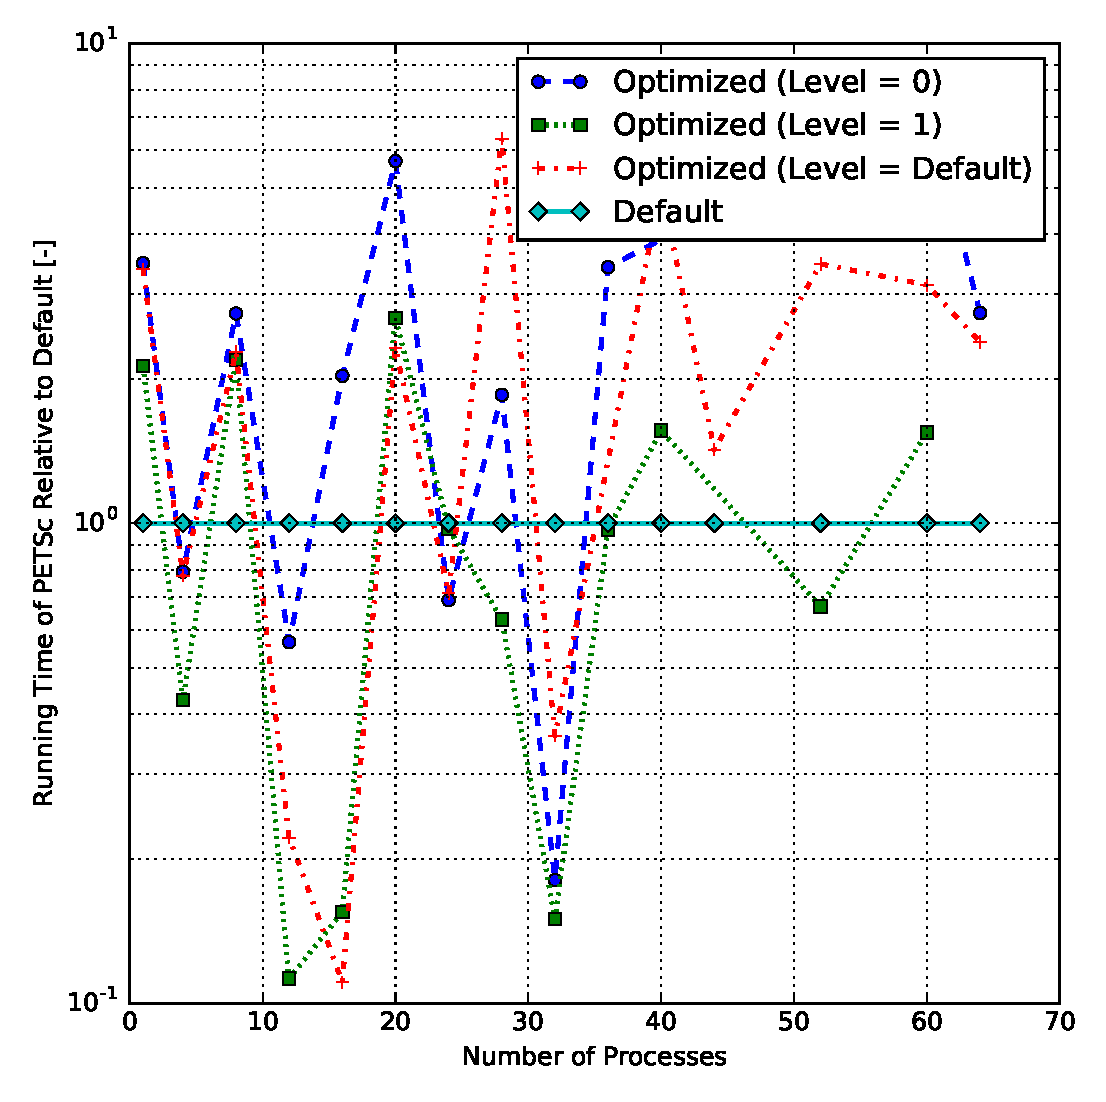
\includegraphics[width=\textwidth]{petsc/laminar-256x64}
      \caption{256x64}
    \end{subfigure}
    \hfill
    \begin{subfigure}{0.45\textwidth}
      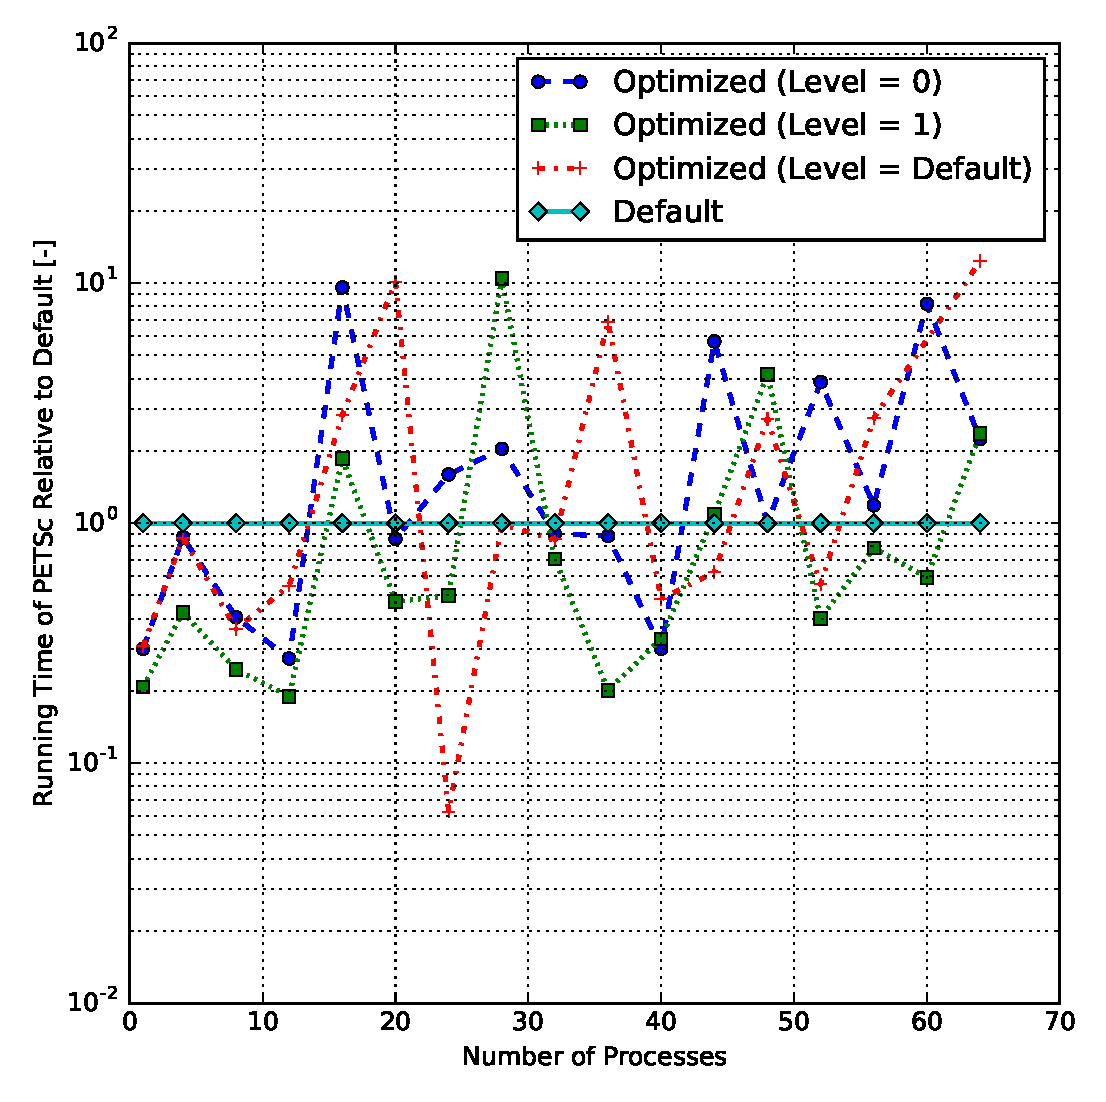
\includegraphics[width=\textwidth]{petsc/laminar-512x128}
      \caption{512x128}
    \end{subfigure}
  \end{figure}
\end{frame}

\begin{frame}
  \frametitle{Scale Testing an Algebraic Turbulence Case}
  \begin{figure}[h]
    \centering
    \begin{subfigure}{0.45\textwidth}
      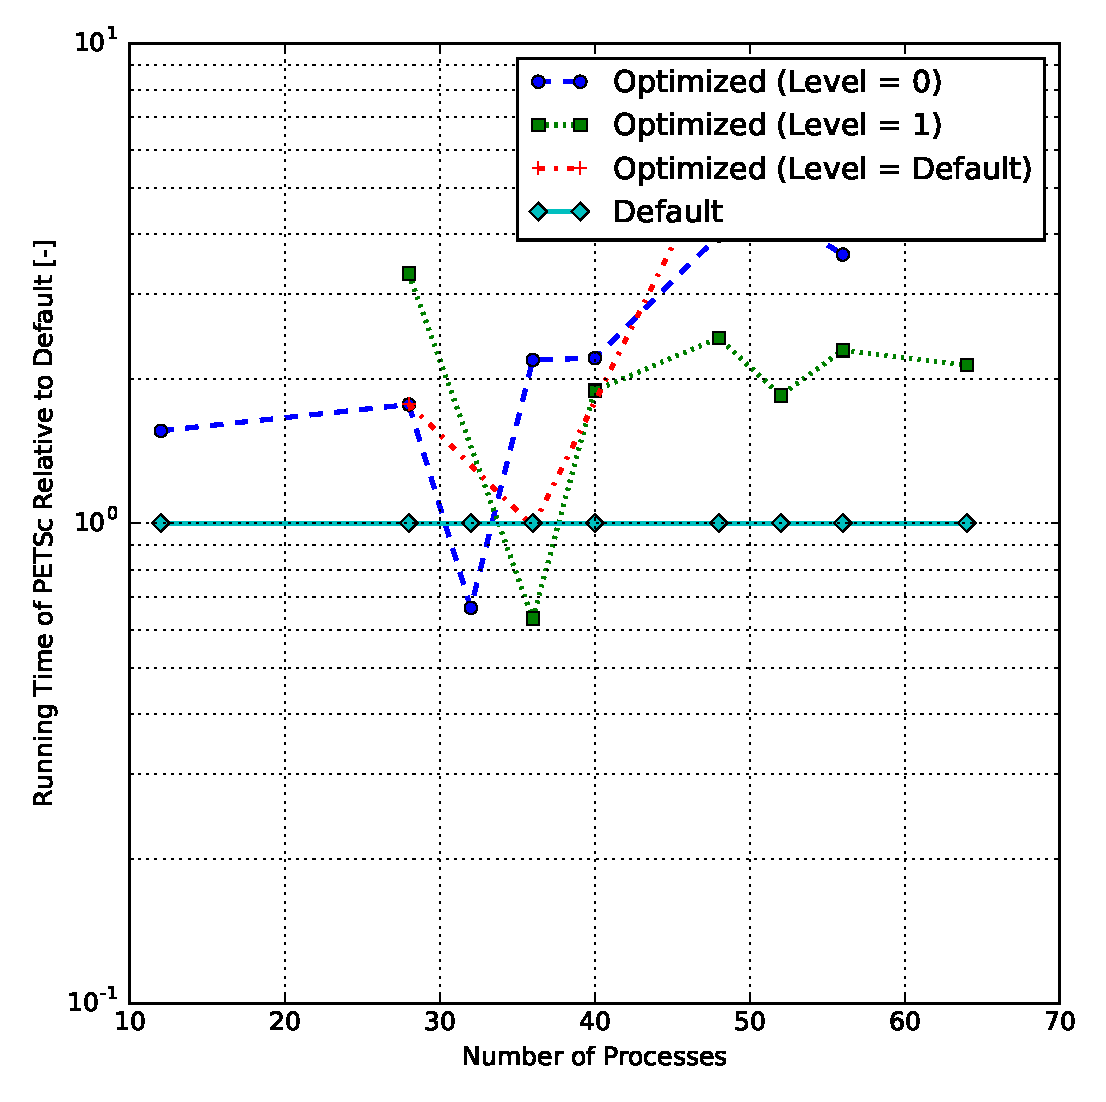
\includegraphics[width=\textwidth]{petsc/algebraic-256x64}
      \caption{256x64}
    \end{subfigure}
    \hfill
    \begin{subfigure}{0.45\textwidth}
      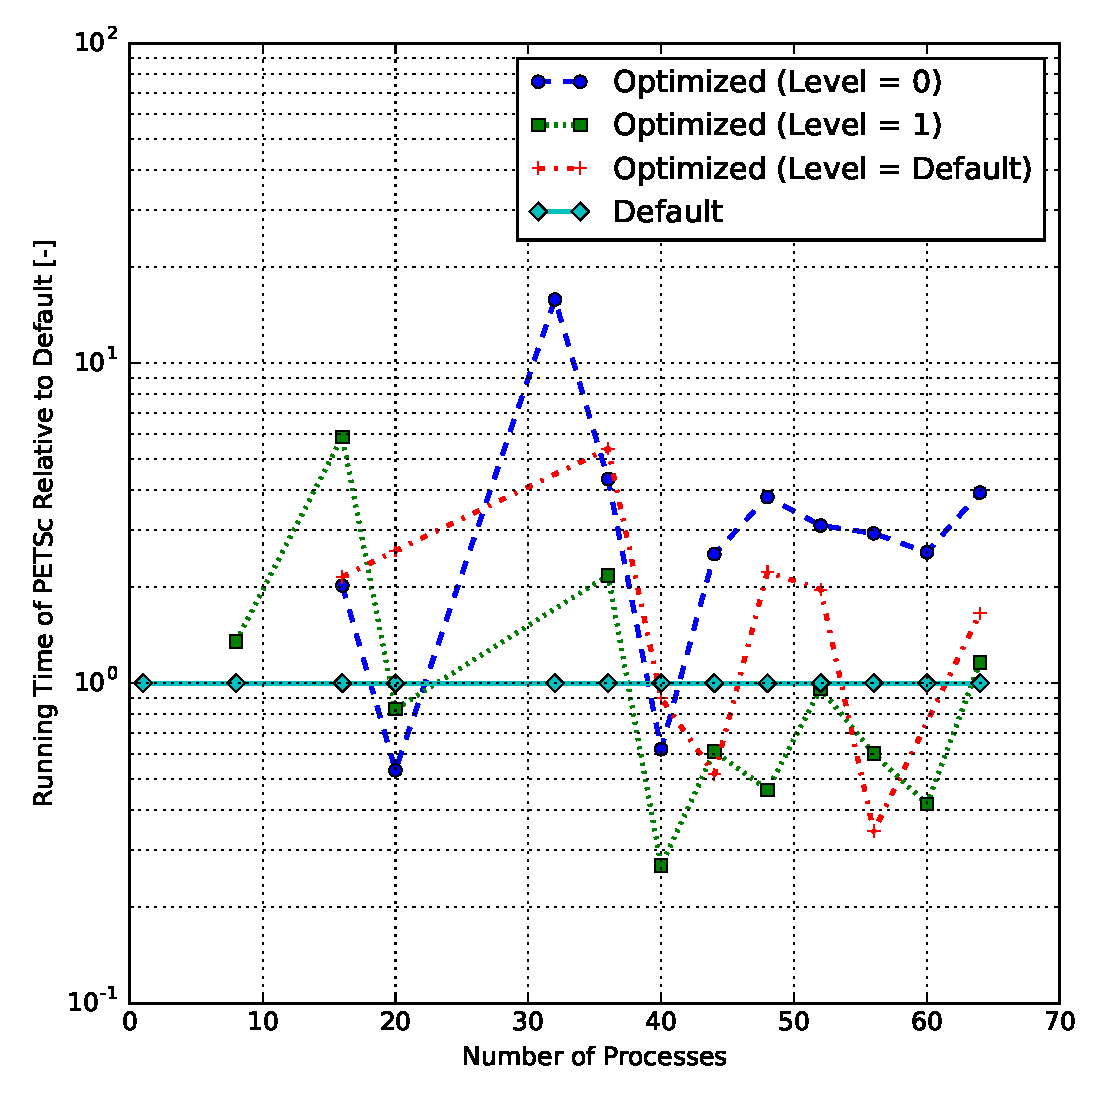
\includegraphics[width=\textwidth]{petsc/algebraic-512x128}
      \caption{512x128}
    \end{subfigure}
  \end{figure}
\end{frame}

\section{Automatic Domain Decomposition}

\end{document}
